\newpage
\subsection{Erzwungene Schwingung}
\index{schwingung!erzwungen}

\begin{figure}[!h]
\centering
\subfloat[Erzwungener Parallel-Schwingkreis]{
	\tikzexternaldisable
\begin{circuitikz}[scale=2, european, american inductors, american currents]
\ctikzset{voltage/european label distance=2}
\ctikzset{bipoles/length=1.2cm}
	\draw
	(0,0)
		to[short](1,0)
		to[short, *-](2,0)
		to[short, *-](3,0)
	(0,0) to[isourcesin, i=$I$] (0,-1)
	(1,0) to[L=L, i>^=$i_L$](1,-1)
	(2,0) to[R=R, i>^=$i_R$](2,-1)
	(3,0) to[C=C, i>^=$i_C$](3,-1)
		to[short, -*](2,-1)
		to[short, -*](1,-1)
		to[short](0,-1);
\end{circuitikz}
\tikzexternalenable
	\label{fig:schwingkreise:erzwungener:parallel}
}
\qquad
\subfloat[I und U im Schwingkreis]{
	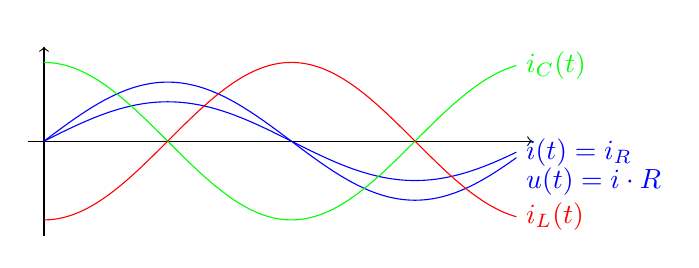
\begin{tikzpicture}[domain=0:6]
	
	\draw[->] (-0.2,0) -- (6.2,0) node[right] {};
	\draw[->] (0,-1.2) -- (0,1.2) node[above] {};
	\draw[color=blue, samples=150]   plot (\x,{0.5*sin(\x r)})   node[right]
	{$i(t)=i_R$};
	\draw[color=blue, samples=150]   plot (\x,{0.75*sin(\x r)})   node[below right]
	{$u(t)=i\cdot R$};
	\draw[color=green, samples=150]   plot (\x,{cos(\x r)})   node[right]
	{$i_C(t)$};
	\draw[color=red, samples=150]   plot (\x,{-1*cos(\x r)})  
	node[right] {$i_L(t)$};
\end{tikzpicture} 
	\label{fig:schwingkreise:erzwungener:sinus} 
}
\caption{Erzwungener Schwingkreis}
\label{fig:schwingkreise:erzwungene}
\end{figure}

% \begin{multicols}{2}
% \begin{wrapfigure}{l}{0.5\textwidth}
% 	\centering
% 	\tikzexternaldisable
\begin{circuitikz}[scale=2, european, american inductors, american currents]
\ctikzset{voltage/european label distance=2}
\ctikzset{bipoles/length=1.2cm}
	\draw
	(0,0)
		to[short](1,0)
		to[short, *-](2,0)
		to[short, *-](3,0)
	(0,0) to[isourcesin, i=$I$] (0,-1)
	(1,0) to[L=L, i>^=$i_L$](1,-1)
	(2,0) to[R=R, i>^=$i_R$](2,-1)
	(3,0) to[C=C, i>^=$i_C$](3,-1)
		to[short, -*](2,-1)
		to[short, -*](1,-1)
		to[short](0,-1);
\end{circuitikz}
\tikzexternalenable
% 	\caption{Erzwungener Parallel-SK}
% 	\label{fig:Schwingkreise:parallel:erzwungen}
% 	\end{wrapfigure}
% \begin{wrapfigure}{r}{0.5\textwidth}
% 	\centering
% 	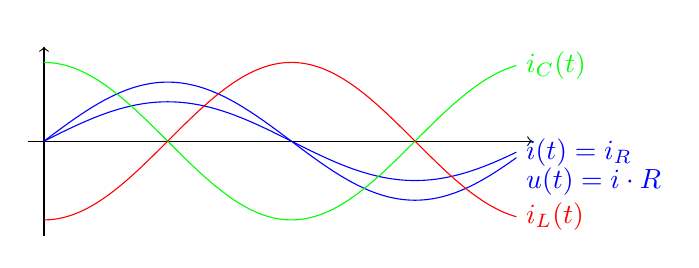
\begin{tikzpicture}[domain=0:6]
	
	\draw[->] (-0.2,0) -- (6.2,0) node[right] {};
	\draw[->] (0,-1.2) -- (0,1.2) node[above] {};
	\draw[color=blue, samples=150]   plot (\x,{0.5*sin(\x r)})   node[right]
	{$i(t)=i_R$};
	\draw[color=blue, samples=150]   plot (\x,{0.75*sin(\x r)})   node[below right]
	{$u(t)=i\cdot R$};
	\draw[color=green, samples=150]   plot (\x,{cos(\x r)})   node[right]
	{$i_C(t)$};
	\draw[color=red, samples=150]   plot (\x,{-1*cos(\x r)})  
	node[right] {$i_L(t)$};
\end{tikzpicture} 
% 	\caption{I und R im Erzwungenen SK}
% 	\label{fig:I-RErzwungen}
% 	\end{wrapfigure}
% \end{multicols}

\begin{wrapfigure}{l}{0.5\textwidth}
	\centering
	\pgfmathdeclarefunction{gauss}{2}{%
  \pgfmathparse{1/(#2*sqrt(2*pi))*exp(-((x-#1)^2)/(2*#2^2))}%
}

\makebox{\begin{tikzpicture}[scale=0.6, every node/.style={scale=0.6}]
\begin{axis}[
  no markers,
  domain=0:6,
  samples=500,
  hide x axis=true,
	hide y axis=true,
  %height=5cm, width=12cm,
  %xtick={4,6.5}, ytick=\empty,
  enlargelimits=false,
  clip=false,
  axis on top,
  grid = major
  ]
  \addplot {gauss(3,1)};
\end{axis}

	\draw[->, thick] (-0.2,0) -- +(right:7.5) node[right] {$t$};
	\draw (3.43,0) node[anchor=north] {$\Delta t$};

	\draw[->, thick] (0,-0.2) -- +(north:6.5) node[above] {$\underline{Z}$};
	\draw (0.05,3.85) -- (-0.05,3.85) node[anchor=east] {$\frac{R}{\sqrt{2}}$};
	\draw (0.05,5.7) -- (-0.05,5.7) node[anchor=east] {$R$};

	\draw[dashed] (0,3.85) -- (4.5,3.85);
	\draw[dashed] (0,5.7) -- (3.55,5.7);
	\draw[dashed, shorten <= -3pt,] (2.43,4) -- (2.43,0);
	%\draw[dashed, shorten <= -3pt] (3.43,5.75) -- (3.43,0);
	\draw[dashed, shorten <= -3pt] (4.43,4) -- (4.43,0);


\end{tikzpicture}}

	\caption{t-Z-Diagramm}
	\label{fig:tZDiagramm}
\end{wrapfigure}



Resonanz: $\omega = \omega_r$\\
\begin{align}
	\underline{Y}_C +\underline{Y}_L &= 0\nonumber\\
	j\omega C+\frac{1}{j\omega L} &= 0\nonumber\\
	\omega=\omega_r&=\frac{1}{\sqrt{LC}}\nonumber\\
	I_C&=U\cdot\omega_rC=I\cdot R \cdot \omega_rC=I\cdot R
	\frac{C}{\sqrt{LC}}\nonumber\\
	&=I\cdot R \sqrt{\frac{C}{L}} = I \cdot Q\nonumber\\
	I_L&=\frac{U}{\omega_rL}=I \cdot Q\nonumber\\
	\omega_r&=\frac{1}{\sqrt{LC}}\nonumber\\
	\frac{f_r}{\Delta f}=\frac{\omega_r}{\Delta \omega} &= Q\nonumber
\end{align}\\


  
\subsubsection{Parallelschwingkreis}
$$\underline{Z} = \frac{1}{\frac{1}{j\omega L}+\frac{1}{R} + j \omega C}
= \frac{j\omega L}{1+j\omega \frac{L}{R}+(j\omega)^2LC}
= \frac{R}{1+(\frac{1}{j\omega L}+j\omega C)R}$$\\
normiert:\\
\begin{align}
\frac{\underline{Z}}{R}&=\frac{1}{1+j(\omega C-\frac{1}{\omega L})\cdot R}
=\frac{j\omega \frac{L}{R}}{1+j\omega\frac{L}{R}+(j\omega)^2LC}\nonumber\\
&=\frac{1}{\sqrt{1+(\omega C - \frac{1}{\omega
L})^2R^2}} \angle \arctan{((\frac{1}{\omega L}-\omega C)\cdot R)} \nonumber
\end{align}\\

Frequenzgang von $\underline Z$:\\
\begin{align}
	\text{Spez. Pt.}&&
	\operatorname{Im}{\{Z\}} = 0 \rightarrow \omega =
	\omega_r=\frac{1}{\sqrt{LC}}\nonumber\\ && Z = Z_{max} = R\nonumber\\
	\text{Tiefe Frequenzen} &&
	\omega \ll \omega_r: \frac{\underline Z}{R} \approx
	j\omega\frac{L}{R}=\omega\frac{L}{R} \angle +90^\circ induktiv\nonumber\\ && \omega \gg \omega_r: \frac{\underline Z}{R} \approx \frac{1}{j\omega RC}
	\angle -90^\circ kapazitiv\nonumber\\
	\text{3dB-Pt} &&
	\frac{Z}{R}=\frac{1}{\sqrt{2}}\nonumber\\
	&& \frac{1}{1+(\omega C-\frac{1}{\omega L})^2R^2}=\frac{1}{2}\nonumber
\end{align}\\

\begin{wrapfigure}{l}{0.5\textwidth}
	\centering
	\pgfmathdeclarefunction{gauss}{2}{%
  \pgfmathparse{1/(#2*sqrt(2*pi))*exp(-((x-#1)^2)/(2*#2^2))}%
}

\makebox{\begin{tikzpicture}[scale=0.7, every node/.style={scale=1.3}]
\begin{axis}[
  no markers,
  domain=0:6,
  samples=500,
  hide x axis=true,
	hide y axis=true,
  %height=5cm, width=12cm,
  %xtick={4,6.5}, ytick=\empty,
  enlargelimits=false,
  clip=false,
  axis on top,
  grid = major
  ]
  \addplot {gauss(3,1)};
\end{axis}

	\draw[->, thick] (-0.2,0) -- +(right:7.5) node[right] {$t$};
	\draw (3.43,0) node[anchor=north] {$\omega_r$};
		\draw[dashed] (3.43,0) -- +(0,6);
	\draw (2.43,0) node[anchor=north] {$\omega_1$};
	\draw (4.43,0) node[anchor=north] {$\omega_2$};

	\draw[->, thick] (0,-0.2) -- +(north:6.5) node[above] {$\underline{Z}$};
	\draw (0.05,3.85) -- (-0.05,3.85) node[anchor=east] {$\frac{R}{\sqrt{2}}$};
	\draw (0.05,5.7) -- (-0.05,5.7) node[anchor=east] {$R$};

	\draw[dashed] (0,3.85) -- (4.5,3.85);
	\draw[dashed] (0,5.7) -- (3.55,5.7);
	\draw[dashed, shorten <= -3pt,] (2.43,4) -- (2.43,0);
	%\draw[dashed, shorten <= -3pt] (3.43,5.75) -- (3.43,0);
	\draw[dashed, shorten <= -3pt] (4.43,4) -- (4.43,0);
	\draw[<->] (4.5,4) -- (4.5,5.75) node[below right] {$3dB$};


\end{tikzpicture}}

	\caption{3dB-Punkt}
	\label{fig:3dBPunkt}
\end{wrapfigure}
\begin{align}
	(\omega C-\frac{1}{\omega L})^2R^2 &= 1\nonumber\\
	(\omega C - \frac{1}{\omega L})R &= \pm 1\nonumber\\
	\omega C - \frac{1}{\omega L} &= \pm \frac{1}{R}\nonumber\\
	\omega^2 \pm \omega \frac{1}{RC}-\frac{1}{LC} &= 0\nonumber\\
	\omega^2 + \frac{\omega_r}{Q}\cdot \omega - \omega_r^2&=0\ bzw\ \omega^2 -
	\frac{\omega_r}{Q}\cdot \omega - \omega_r^2=0\nonumber
	\omega_{1,1,2} = -\frac{\omega_r}{2Q} \pm 
	\underbrace{\omega_r\sqrt{\frac{1}{4Q^2}+1}}_{>\frac{\omega_r}{2Q}}
	\	bzw\ \omega_{2,1,2}=\frac{\omega_r}{2Q} \pm
	\underbrace{\omega_r\sqrt{\frac{1}{4Q^2}+1}}_{>\frac{\omega_r}{2Q}} \nonumber\\
\end{align}
%geschwoffene klammern unten dran mechen //TODO


3dB Frequenzgrenzen:\\
\begin{align}
\boxed{\omega_{1,2}=\omega_r(\sqrt{\frac{1}{4Q^2}+1}\mp\frac{1}{2Q})}
\end{align}
